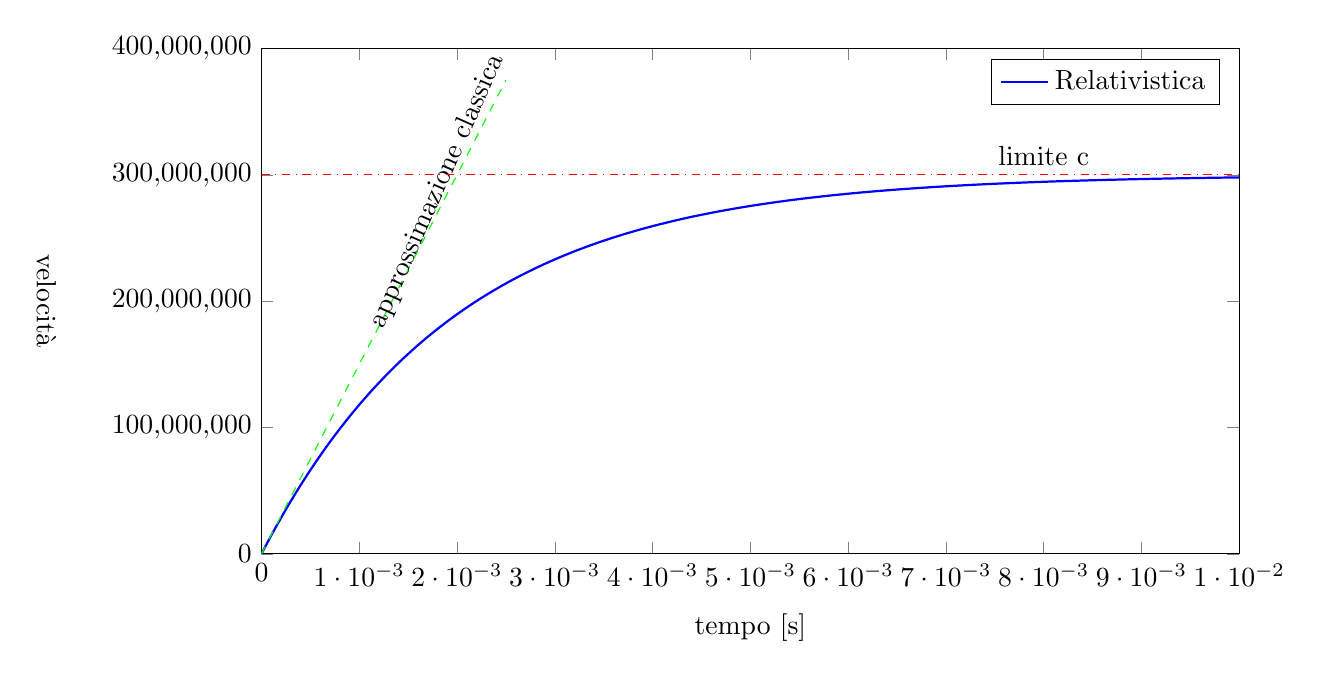
\begin{tikzpicture}
\begin{axis}[
    width=14cm,
    height=8cm,
    xlabel={tempo [s]},
    ylabel={velocità},
    xmin=0, xmax=0.01,
    ymin=0, ymax=4e8,
    xtick={0,0.001,0.002,0.003,0.004,0.005,0.006,0.007,0.008,0.009,0.01},
    yticklabel style={/pgf/number format/fixed},
    scaled y ticks=false,
    scaled x ticks=false,
    y label style={at={(axis description cs:-0.2,.5)},rotate=180},
    x label style={at={(axis description cs:0.5,-0.1)}},
]

% Parametri
\def\c{3e8} % velocità della luce
\def\a{1.5e11} % accelerazione costante (esempio)

% Curva relativistica (approssimazione)
\addplot[blue, thick, domain=0:0.01, samples=200] 
    {\c*(1 - exp(-\a*x/\c))}; % modello esponenziale per saturazione
\addlegendentry{Relativistica}

% Curva classica
\addplot[green, dashed, domain=0:0.0025, samples=100] 
    {\a*x};
\node[above, rotate=66] at (axis cs:0.002,2.8e8) {approssimazione classica};

% Linea limite c
\addplot[red, dash dot, domain=0:0.01] {\c};
\node[above] at (axis cs:0.008,3e8) {limite c};

\end{axis}
\end{tikzpicture}
